% ============================================================
% Chapter 4: Estimator Properties
% ============================================================
\chapter{Estimator Properties --- Bias, Consistency, Efficiency}
\label{ch:properties}

\begin{center}
\textit{``A good estimator should aim true and not scatter too much.''}
\end{center}

\section{Motivating Example}

Two shooters aim at a target. The first hits the center on average but is scattered. The second clusters tightly but consistently to the right. Who is ``better''? This is the bias-variance tradeoff.

\section{Bias}

\begin{definition}[Bias]
\index{bias}
$\Bias(\thetahat) = \E_\theta[\thetahat] - \theta$. The estimator is \textbf{unbiased} if $\Bias(\thetahat)=0$ for all $\theta$.
\end{definition}

\begin{proposition}
$S^2=\frac{1}{n-1}\sum(X_i-\xbar)^2$ is unbiased for $\sigma^2$.
\end{proposition}

\begin{proof}
$\E[\sum(X_i-\xbar)^2]=n(\sigma^2+\mu^2)-n(\sigma^2/n+\mu^2)=(n-1)\sigma^2$.
\end{proof}

\section{Mean Squared Error}

\begin{definition}[MSE]
\index{MSE}\index{mean squared error}
$\MSE(\thetahat) = \E_\theta[(\thetahat-\theta)^2]$.
\end{definition}

\begin{theorem}[Bias-Variance Decomposition]
\label{thm:bias-variance}
$\MSE(\thetahat) = \Var(\thetahat) + [\Bias(\thetahat)]^2$.
\end{theorem}

\begin{proof}
Let $b=\E[\thetahat]-\theta$. Then $\MSE = \E[(\thetahat-\E[\thetahat]+b)^2] = \Var(\thetahat)+b^2$.
\end{proof}

\begin{intuition}
MSE combines two error sources. A biased estimator can have lower MSE than an unbiased one if its variance is sufficiently reduced. This is the \textbf{bias-variance tradeoff}, fundamental in statistical learning.
\end{intuition}

\begin{center}
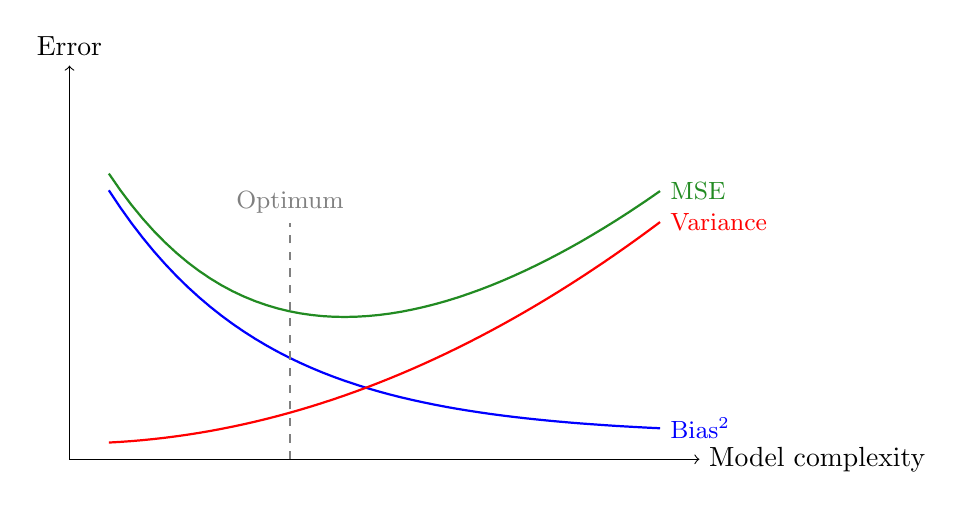
\begin{tikzpicture}
\draw[->] (0,0) -- (8,0) node[right] {Model complexity};
\draw[->] (0,0) -- (0,5) node[above] {Error};
\draw[thick,blue,domain=0.5:7.5,samples=50] plot (\x, {4*exp(-0.5*\x)+0.3}) node[right] {\small Bias$^2$};
\draw[thick,red,domain=0.5:7.5,samples=50] plot (\x, {0.05*\x*\x+0.2}) node[right] {\small Variance};
\draw[thick,ForestGreen,domain=0.5:7.5,samples=50] plot (\x, {4*exp(-0.5*\x)+0.05*\x*\x+0.5}) node[right] {\small MSE};
\draw[dashed,gray] (2.8,0) -- (2.8,3) node[above] {\small Optimum};
\end{tikzpicture}
\end{center}

\section{Consistency}

\begin{definition}[Consistent Estimator]
\index{consistency}
$\thetahat_n$ is \textbf{consistent} if $\thetahat_n \xrightarrow{\Prob} \theta$.
\end{definition}

\begin{proposition}
If $\Bias(\thetahat_n)\to 0$ and $\Var(\thetahat_n)\to 0$, then $\thetahat_n$ is consistent.
\end{proposition}

\section{Efficiency and Cram\'er--Rao Bound}

\begin{theorem}[Cram\'er--Rao Inequality]
\index{Cramer-Rao@Cram\'er--Rao}
\label{thm:cramer-rao}
Under regularity conditions, for any unbiased estimator $\thetahat$ of $g(\theta)$:
\[
\Var_\theta(\thetahat) \geq \frac{[g'(\theta)]^2}{nI(\theta)}.
\]
\end{theorem}

\begin{proof}
By Cauchy--Schwarz. Let $V=\sum\frac{\partial}{\partial\theta}\ln f(X_i;\theta)$ (total score). Then $\E[V]=0$, $\Var(V)=nI(\theta)$, and $\Cov(\thetahat,V)=g'(\theta)$. So $[g'(\theta)]^2\leq\Var(\thetahat)\cdot nI(\theta)$.
\end{proof}

\begin{definition}[Efficient Estimator]
\index{efficiency}
$\thetahat$ is \textbf{efficient} if it attains the Cram\'er--Rao bound.
\end{definition}

\begin{example}
For $X_i\iid\mathcal{N}(\mu,\sigma^2)$ ($\sigma^2$ known): $\Var(\xbar)=\sigma^2/n=1/(nI(\mu))$. So $\xbar$ is efficient.
\end{example}

\section{UMVUE and Rao--Blackwell}

\begin{theorem}[Rao--Blackwell]
\index{Rao--Blackwell}
If $\thetahat$ is unbiased for $g(\theta)$ and $T$ is sufficient, then $\thetahat^*=\E[\thetahat\mid T]$ is unbiased with $\Var(\thetahat^*)\leq\Var(\thetahat)$.
\end{theorem}

\begin{theorem}[Lehmann--Scheff\'e]
\index{Lehmann--Scheffe@Lehmann--Scheff\'e}
If $T$ is sufficient and complete, then any unbiased estimator that is a function of $T$ is UMVUE.
\end{theorem}

\section{Python Implementation}

\begin{python}
\begin{minted}{python}
import numpy as np
import matplotlib.pyplot as plt

np.random.seed(42)
sigma2_true = 4; n = 10; n_sim = 50000

biased = np.array([np.var(np.random.normal(0, 2, n), ddof=0) for _ in range(n_sim)])
unbiased = np.array([np.var(np.random.normal(0, 2, n), ddof=1) for _ in range(n_sim)])

print(f"MLE (n):  E={np.mean(biased):.4f}, MSE={np.mean((biased-sigma2_true)**2):.4f}")
print(f"S^2 (n-1): E={np.mean(unbiased):.4f}, MSE={np.mean((unbiased-sigma2_true)**2):.4f}")
print(f"Cramer-Rao bound for mu: {sigma2_true/n:.4f}")

fig, ax = plt.subplots(figsize=(8, 5))
ax.hist(biased, bins=50, alpha=0.5, density=True, label='MLE (n)')
ax.hist(unbiased, bins=50, alpha=0.5, density=True, label='$S^2$ (n-1)')
ax.axvline(sigma2_true, color='red', lw=2, label=f'$\\sigma^2={sigma2_true}$')
ax.legend(); ax.set_title(f'Estimators of $\\sigma^2$ (n={n})')
plt.savefig("ch04_bias_variance.pdf"); plt.show()
\end{minted}
\end{python}

\section{Exercises}

\begin{exercise}[$\star$]
Is $\hat{\lambda}=1/\xbar$ unbiased for $\lambda$ when $X_i\iid\mathrm{Exp}(\lambda)$?
\end{exercise}

\begin{exercise}[$\star\star$ -- Cram\'er--Rao]
Show that $\xbar$ attains the CR bound for $p$ in $\mathrm{Bernoulli}(p)$.
\end{exercise}

\begin{exercise}[$\star\star$ -- Rao--Blackwell]
For $X_i\iid\mathrm{Pois}(\lambda)$, improve $\thetahat=\mathbf{1}_{X_1=0}$ as an estimator of $e^{-\lambda}$ using $T=\sum X_i$.
\end{exercise}

\begin{exercise}[$\star\star$ -- Bias-variance tradeoff]
For $\thetahat_c=c\cdot S^2$ estimating $\sigma^2$, find the $c^*$ minimizing MSE.
\end{exercise}

\begin{exercise}[$\star\star\star$ -- Project]
Verify numerically that $\xbar$ is efficient for Poisson$(\lambda)$. Compare MSE of mean, median, and sample variance as estimators of $\lambda$.
\end{exercise}

\begin{keyformulas}
\begin{align*}
\Bias(\thetahat) &= \E[\thetahat]-\theta \\
\MSE(\thetahat) &= \Var(\thetahat)+[\Bias(\thetahat)]^2 \\
\text{CR bound} &: \Var(\thetahat)\geq \frac{[g'(\theta)]^2}{nI(\theta)} \\
\text{Rao--Blackwell} &: \thetahat^*=\E[\thetahat\mid T],\;\Var(\thetahat^*)\leq\Var(\thetahat)
\end{align*}
\end{keyformulas}
